\documentclass{scrreprt}
\usepackage{listings}
\usepackage{underscore}
\usepackage[francais]{babel}
\usepackage[utf8]{inputenc}
\usepackage[bookmarks=true]{hyperref}
\usepackage{tabularx}
\usepackage{graphicx}
\usepackage{hyperref}

\hypersetup{
    bookmarks=false, % show bookmarks bar?
    pdftitle={Document de spécification des exigences du logiciel}
	pdfauthor={Jean-Philippe Caissy\\Stéphan Michaud\\Guillaume Auger\\Maxime
		Bélanger\\Justin Michaud-Ouelette\\Frédéric Sevillano}
	pdfsubject={TeX and LaTeX}, % subject of the document %pdfkeywords={TeX, LaTeX, graphics, images}, % list of keywords
    colorlinks=true, % false: boxed links; true: colored links
    linkcolor=blue, % color of internal links
    citecolor=black, % color of links to bibliography
    filecolor=black, % color of file links
    %urlcolor=purple, % color of external links
    linktoc=page % only page is linked
}
\def\myversion{1.0 }
\title{
\flushright
\rule{16cm}{5pt}\vskip1cm
\Huge{Document de spécification des exigences du logiciel}\\
\vspace{2cm}
pour\\
\vspace{2cm}
Nitcorn\\
\vspace{2cm}
%\LARGE{Release 1.0\\}
%\vspace{2cm}
%\LARGE{Version \myversion approved\\}
%\vspace{2cm}
Préparé par Jean-Philippe Caissy\\Stéphan Michaud\\Guillaume Auger\\Maxime
Bélanger\\Justin Michaud-Ouelette\\Frédéric Sevillano\\
\vfill
\rule{16cm}{5pt}
}
\date{}
\begin{document}
\maketitle
\tableofcontents
\chapter*{Historique de révision}
\begin{tabularx}{\textwidth}{|r|X|r|}
    \hline
    Nom & Description & Date \\
    \hline
    Stéphan Michaud & Création & 2013/02/04 \\
    \hline
    Équipe & Ébauche & 2013/02/26 \\
    \hline
    Jean-Philippe Caissy & Conversion en \LaTeX & 2013/03/04 \\
    \hline
    Jean-Philippe Caissy,& Fonctionalités & 2013/03/24\\
    Stéphan Michaud,& &\\
    Justin Michaud-Ouelette, & &\\
    Frédéric Sevillano & & \\
    \hline
    Maxime Bélanger & Règler quelques problèmes & 2013/03/27  \\
    \hline
    Guillaume Auger & Correction de l'orthographe & 2013/03/28  \\
     & Modification des acteurs &\\
     & Modifications aux définitions &\\
    \hline
    Équipe & Rédaction de groupe & 2013/04/11 \\
    \hline
    Maxime Bélanger & Définition & 2013/04/13 \\
    \hline
    Guillaume Auger & Souligner les parties à compléter/corriger & 2013/04/16 \\
    \hline
    Guillaume Auger & Terminer headers & 2013/04/18 \\
    & Description des méthodes & \\
    & Contraintes sur la base de données & \\
    & Conformité avec les standards & \\
    \hline
\end{tabularx}

\chapter{Introduction}
Ce chapitre permet d'introduire la documentation du serveur Internet Nitcorn. Il permettra d'éliminer toute ambiguïté concernant la documentation
de notre application à l'aide de définitions, acronymes et
abréviations. Les objectifs et les portées seront décrits pour
avoir une meilleure compréhension du document.
\section{Objet}
L'objectif de ce document est de présenter une description complète, détaillée et précise des exigences de l'application Nitcorn. Le concept des exigences sera décrit textuellement et différents types de diagrammes seront utilisé pour illustrer l'interaction avec l'utilisateur. De plus, une spécification d'interface externe sera décrite permettant aux applications Nit existantes d'utiliser un serveur web.\\

Ce document s'adresse aux développeurs du projet Nitcorn ainsi qu'aux potentiels
contributeurs externes.
\section{Portée}
L'application décrite par le présent document se nomme Nitcorn. Elle sera responsable d'offrir un serveur web aux applications Nit. Étant un nouveau language de programmation développé principalement par un professeur de l'UQAM, Nit n'a pas encore de librairie capable d'établir une connexion entre une application et un serveur web. Le but de cette application est d'en offrir la possibilité. Le document sera composé d'une description des différentes composantes que le serveur va offrir à l'usager. Voici ces fonctionnalités:
\begin{itemize}
    \item Écoute sur un socket;
    \item Réception de requêtes HTTP 1.0 et 1.1;
    \item Traitement et réponse à une requête HTTP;
    \item Exposer une API pour gérer la configuration;
    \item Gestion de log;
    \item Transmettre les requêtes vers un serveur mandataire;
    \item Permettre la ré-écriture des requêtes HTTP;
    \item Chiffrement et déchiffrement (SSL/TLS);
    \item Persistance de la configuration;
\end{itemize}

\section{Définitions, acronymes et abréviations}
Voici les définitions des différents termes techniques utilisés dans ce
document.
\begin{description}
    \item[Apache] Serveur Web connu pour jouer un rôle clé dans la croissance initiale du World Wide Web.
	\item[API] Interface qui rend possible l'interaction entre un homme et une machine.
    \item[Asynchrone]Technique permettant de mettre en oeuvre des opérations qui sont exécutées simultanément, mais non syncronisées entre elles, avec le reste du programme. 
	\item[Authentification Basic]Technique de base pour renforcer les contrôles d'accès aux ressources Web.
    \item[Authentification Digest]Technique plus sécuritaire pour renforcer les contrôles d'accès aux ressources Web.
	\item[Boucle d'événement asynchrone] Structure de programmation qui attend et distribue les événements ou les messages de façon asynchrone dans un programme.
    \item[Contenu] Information binaire.
    \item[Cookie HTTP] Petit contenu envoyé par un site web et stocké par le client. Le contenu peut par la suite être récupéré par le serveur lors d'une prochaine visite.
    \item[Domaine] Fully qualified domain name. Nom qualifiant un et un seul emplacement dans les trois hiérarchies du DNS.
    \item[DNS] Domain Name System. Associe les domaines aux adresses IP.
    \item[Fastcgi] Protocole d'interface de programmes interactifs avec un serveur Web. 
    \item[Fil d'éxécution] Traitement d'une suite d'instructions par la machine sur un programme donné.
    \item[File descriptor] Identifiant d'un fichier ouvert par le système d'exploitation. 
 	\item[Header] Les en-têtes retrouvées dans les requêtes et les réponses HTTP/1.0 et HTTP/1.1
    \item[Host] Identifiant de domaine internet.	
	\item[HTTP 1.0] Version 1.0 du protocole HTTP. Ne permet pas de connexions de type keep-alive.
	\item[HTTP 1.1] Version 1.1 du protocole HTTP qui support d'avantage de méthodes et d'en-têtes que la version 1.0
    \item[Itanium] Processeurs 64 bits développés par Intel utilisant l'architecture IA_64. Inclus ici les processeurs Itanium 2.
	\item[Log] Désigne un historique d'événements (Journal des événements).   
    \item[Méthode HTTP] Intention de la requête.
	\item[MIME] Multipurpose Internet Mail Extensions. Est un identifiant de format de données composé de deux parties, utilisé par les serveurs pour distinguer le type de format.
	\item[Nit] Langage de programmation open source orienté objet développé par le
groupe de recherche sur l'étude, la spécification et l'implémentation des
langages informatique du département d'informatique à l'Université du Québec à
Montréal.
	\item[Nginx] Serveur asynchrone où chaque requête est traitée par un processus dédié.   
	\item[Protocole HTTP] Protocole de communication applicative d'architecture
client-serveur\cite{http}.
	\item[Requête HTTP] Demande envoyée par le client au serveur via un réseau.
Connexion keep-alive\cite{http1.0}.
	\item[Reverse Proxy] Type de serveur, habituellement placé en frontal de serveurs web. Il est à différencier dans son utilisation des serveurs proxys traditionnels.
    \item[Site web] Ensemble de pages web sur un même domaine.
	\item[Socket] Interface logiciel de connexion réseau.   
    \item[SSL] Secure Sockets Layer. Un protocole de sécurisation des échanges sur Internet.
	\item[Standard NCSA Common log format]  Format de journal ne contenant que des informations concernant l'accès HTTP.
    \item[TLS] Transport Layer Security. Un protocole de sécurisation des échanges sur Internet. 
    \item[UQAM] Université du Québec à Montréal.    
    \item[URI] Uniform resource identifier. Chaîne de caractères identifiant une ressource.
    \item[URL] Uniform resource locator. Adresse web qui réfère à une ressource.
    \item[Virtual Host] Ensemble d'hosts dont un serveur est responsable.
    \item[x86] Architecture de processeur 32 bits développée par Intel.
    \item[x86_64] Architecture de processeur 64 bits développée par AMD, mais compatible avec la famille de processeur 64 bits d'Intel (à l'exception de Itanium).

\end{description}

\section{Références}

\begin{tabularx}{\textwidth}{|l|X|l|l|l|}
    \hline
    Ref. & Numéro du document & Titre & Organisation & Date\\
    \hline
    \cite{ieefr} & IEEE 830-& Norme IEEE 830-1993 & Institute of Electrical and & 1993\\
    & 1993& &  Electronics Engineers &\\
    \hline
    \cite{http} & RFC2616 & Hypertext Transfer Protocol & The Internet Society&	1999\\
    & & -- HTTP/1.1& &\\
    \hline
    \cite{NCSA} & N/A & NCSA Common Log Format & NCSA & N/A \\
    \hline
\end{tabularx}

\section{Vue d'ensemble}
Le  reste du document va contenir toutes les exigences de notre application organisées sous différentes sections.
\\
\\
La section 2 va contenir les facteurs généraux qui vont influencer le produit et ses exigences. Une description des différents modules du système sera présentée. Cette section traitera les aspects suivants:
\begin{description}
\item[Description] Description globale du projet et de ses interfaces.
\item[Récits des fonctions] Récits décrivant une fonction du point de vue de son utilisateur. Organisés par utilisateurs.
\item[Caractéristiques des utilisateurs] Caractéristiques requises par les utilisateurs
\item[Contraintes] Éléments qui risquent de contraindre le développeur.
\item[Hypothèses et dépendances] Facteurs influençants les exigences.
\end{description}

La section 3 va couvrir en détail toutes les exigences du système afin que les concepteurs puissent être en mesure de concevoir le système et satisfaire les exigences du système. Cette section traitera les aspects suivants:

\begin{description}
\item[Exigences spécifiques] Décrit de façon précise les cas d'utilisation.
\item[Contraintes de conception] Contraintes qui doivent être suivies lors de la conception du système.
\item[Attributs] Attributs de logiciel pouvant servir d'exigences. 
\end{description}
\chapter{Description générale}
\section{Environnement}
(@TODO INCLURE UN DIAGRAMME ILLUSTRANT LES INTERFACES?:)\\
(@TODO A block diagram showing the major components of the larger system, interconnections, and external inter-
faces PIJI)

Le but premier de Nitcorn est d'offrir aux applications développés en Nit la possibilitée
d'utiliser un serveur web. On va donc devoir créer un module pour le langage Nit afin que d'autres applications Nit puissent être en mesure d'utiliser un serveur web. Il offrira des fonctionnalités de serveur au langage afin qu'il puisse être placé derrière un serveur web(Nginx, Apache,\ldots). Sous cette configuration, il va pouvoir répondre à des dizaines de milliers de requêtes web par seconde. Un service web sera utilisé afin de configurer le serveur. La gestion des logs ou la persistance des configuration devront être gérés automatiquement par le serveur web.\\ De cette façon, l'utilisateur pourrait avoir accès au log pour déterminer l'état du serveur. De plus, lorsqu'une erreur est détectée, un message d'erreur sera retourné à l'utilisateur. Nitcorn sera directement exposé à Internet et devra agir en tant qu'un serveur web exactement comme c'est le cas pour les autres
serveurs web (Nginx, Apache, \ldots). Sous cette configuration, les
fonctionnalités mentionnées ci-haut doivent être utilisées pour assurer les requis de traçabilité
et de fonctionnalités essentiels au serveur web.

\subsection{Interfaces avec le système}
Nitcorn sera utilisé sur deux systèmes : un serveur web et un environnement de développement.
Le serveur web sera le système ayant comme fonctionnalité d'agir en tant que serveur web, alors
que l'environnement de développement sera le système utilisé par les développeurs
pour développer des applications web en Nit.

\subsubsection{Interface serveur/application}
Pour communiquer avec le serveur, l'application web devra redéfinir la classe HTTPServer pour modifier la méthode answer() qui définit la réponse à la requête. 
La méthode answer() prend en argument une requête http qui est une classe HttpRequest du module http_request, et écrit la réponse http, une sous-classe HttpResponse avec write().\\\\
La réponse http doit être composée de la version du protocole HTTP, du code de status, du texte de status, d'un HashMap contenant les \textit{headers} et leur valeur, ainsi que du corps du texte.\\\\
Voici un exemple simple:\\
On définit la réponse dans la méthode answer():\\
var response = new HttpResponse("HTTP/1.0", 200, "OK", new HashMap[String, String], "Hello world")\\
Puis on la retourne en l'écrivant avec write:\\
write(response.to_s)


\subsection{Interfaces avec les utilisateurs}
Comme il est disponible avec les autres serveurs web, un système de log est
disponible permettant à un utilisateur de déterminer la cause du problème. Sur
un autre point, le logiciel aura une API permettant aux applications Nit de
communiquer sur le web sans avoir à se soucier des configurations. Cette
API sera grandement inspirée par l'interface universelle WGSI développée pour
le langage Python. Le logiciel Nitcorn offrira aussi une interface pour les
applications Nit.

\subsection{Interfaces avec le matériel}
Nitcorn dépend du compilateur de Nit. Celui-ci est compatible pour le moment avec
les architectures x86 et x86_64.

\subsection{Interfaces avec les logiciels}
Nitcorn ne supporte que les systèmes d'exploitation de style UNIX (GNU/Linux, *BSD, Mac OS X, etc).
De plus, Nitcorn a besoin des logiciels suivants lors de la compilation : \\
\\
\begin{tabular}{|l|l|l|l|l|}
    \hline
    Nom & Mnémonique & Spécification & Version & Source \\
    \hline
    Nitc & N/A & FFI & N/A & \url{https://github.com/xymus/nit/tree/ffi} \\
    \hline
    Libevent & N/A & N/A & 2.0.X & \url{http://libevent.org/} \\
    \hline
    SQLite & N/A & DEV & 3.X & \url{https://www.sqlite.org/} \\
    \hline

\end{tabular}

\section{Fonctions}
Les différentes fonctions sont séparées en deux groupes : serveur et application Nit.
Le serveur est Nitcorn, alors que l'application Nit est l'application qui utilise
Nitcorn pour répondre à des requêtes web dynamiquement. De plus, une API est existante pour la gestion des configurations selon les préférences de l'utilisateur.\\
\begin{figure}[ht!]
    \caption{Liens entre les composants}
    \centering
    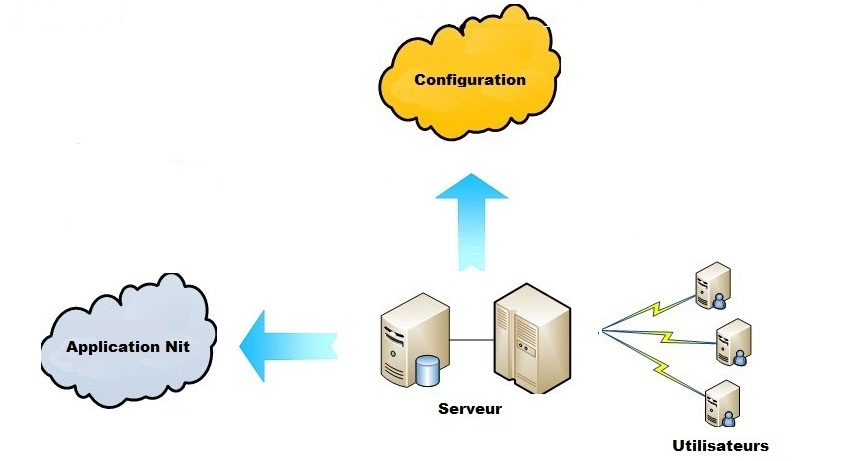
\includegraphics[width=9cm]{diagram/diagram1}
\end{figure}


\subsection{Serveur}
\begin{itemize}
 \item Réception d'une requête
 \item Traiter une requête
 \item Lire la configuration
 \item Écrire la configuration
 \item Enregistrer les événements
\end{itemize}
\subsection{Application Nit}
\begin{itemize}
 \item Recevoir une requête HTTP
 \item Traiter une requête HTTP
\end{itemize}
\subsection{API}
\begin{itemize}
 \item Lire la configuration
 \item Modifier la configuration
 \item Enregistrer la configuration
\end{itemize}
\section{Caractéristiques des utilisateurs}
Les utilisateurs de Nitcorn seront en général soit des développeurs ou des
administrateurs de réseaux. Ce sont des gens qui ont soit une formation de
niveau collégiale ou universitaire ou une expérience professionnelle dans
le domaine du web. Il faudra connaître l'effet de certaines variables de
configuration ou être prêt à lire la documentation qui sera fournie.
Dernièrement, il y aura aussi les clients qui eux feront les requêtes
au serveur.
\section{Contraintes}

\subsection{Mémoire}
Nous n'imposons aucune contrainte mémoire. Par contre, la quantité de
\textbf{file descriptors} ouvert en même temps sera limitée par le noyau du
système d'exploitation. La limite est à la discrétion de l'utilisateur. Le
serveur devra gérer l'atteinte de cette limite.
\subsection{Exécution}
Le traitement des requêtes doit s'effectuer de façon asynchrone sur un seul fil
d'exécution. Plusieurs requêtes doivent être traitables simultanément sans bloquer
les nouvelles requêtes entrantes.
\subsection{Architecture}
Nous avons décidé d'utiliser un patron de conception basé sur
une boucle d’événements pour les communications bloquantes sur les sockets. Cela va 
permettre de n'utiliser qu'un seul processus pour le serveur, tout en restant très performant.
Ce mécanisme permet d'utiliser des mécanismes existant du système d'exploitation
pour gérer de manière asynchrone les entrées et sorties\cite{c10k}.



\subsection{Utilisation du serveur}
La spécification complète et exacte des méthodes, \textit{headers} et des codes de status suivants se retrouvent dans le RFC2616 listé dans les références.
\subsubsection{Le serveur devra supporter les méthodes HTTP/1.0 et HTTP/1.1 suivantes}
\begin{description}
 \item [OPTIONS] Demande les informations sur les options de communication disponible.
 \item [GET] Demande la ressource identifié par l'URI.
 \item [HEAD] Identique à GET, mais la réponse ne doit pas contenir de \textit{message body}.
 \item [POST] Indique que des données sont envoyés dans le \textit{message body} et demande au serveur d'en prendre compte.
 \item [PUT] Demande de stocker les données envoyé par la requête.
 \item [DELETE] Demande d'effacer la ressource identifiée par l'URI.
 \item [TRACE] Invoque les serveurs intermédiaires pour leur demander de lui réenvoyer la requête.
 \item [CONNECT] Demande au serveur d'ouvrir un tunnel TCI/IP.
\end{description}

\subsubsection{Le serveur devra être en mesure de supporter les headers suivants}

\subsubsection{Http/1.0}
\subsubsection{General-Headers:}
        \begin{description}
        \item [Date] La date et l'heure de l'origine du message en format HTTP-date.
        \item [Pragma] Liste de directives supplémentaires d'implémentation.
        \end{description}
\subsubsection{Request-Headers:}
        \begin{description}
        \item [Authorization] Identification du navigateur avec le serveur.
        \item [From] L'adresse e-mail du client.      
        \item [If-Modified-Since] la reqête doit avoir été modifiée depuis la date spécifiée.
        \item [Referer] URL du lien de la requête effectuée.          
        \item [User-Agent] liste d'information sur le client(nom et version)       
        \end{description}
\subsubsection{Response-Headers:}
        \begin{description}
        \item [Location] Redirection vers une nouvelle URL associée au document.           
        \item [Server] Caractéristiques du serveur qui émet la réponse.          
        \item [WWW-Authenticate] Inclue avec une réponse à une erreur d'authentification 401.
        \end{description}
\subsubsection{Entity-Headers:}
        \begin{description}
        \item [Allow] Liste de méthodes supportées par la resource                
        \item [Content-Encoding] Type d'encodage du corps de la requête  
        \item [Content-Length] Longueur du corps de la requête    
        \item [Content-Type] Le type MIME du corps de la requête.      
        \item [Expires] Date d'expiration des données.           
        \item [Last-Modified] La date et l'heure de la dernière modification, en format HTTP-date.     
        \item [Extension-header] L'ajout de headers supplémentaires.
        \end{description}
\subsubsection{Http/1.1}
\subsubsection{General-Headers:}
        \begin{description}
        \item [Cache-Control] Directives imposées au systèmes de cache rencontrés dans la requête et la réponse.      
        \item [Connection] Options des spécifications de la connection courante.     
        \item [Trailer] Liste des headers présent dans le message encodé.          
        \item [Transfer-Encoding] Indique le type de transformation effectuée sur le corps du message afin de se rendre à déstination.
        \item [Upgrade] Spécifie les autres protocoles de communication supportées au server.          
        \item [Via] Doit être utilisé par les passerelles et proxys pour indiquer les protocoles intermédiaires entre le serveur et le client.
        \item [Warning] Contient des information additionnelles sur le status ou la transformation du message.
        \end{description}
\subsubsection{Request-Headers:}
        \begin{description}
        \item [Accept] Spécifie les types de données acceptées dans la réponse.
        \item [Accept-Charset] Indique le codage des caractères accepté dans la réponse.
        \item [Accept-Encoding] Similaire au \textit{Accept}, mais restreint l'encodage du contenu acceptable dans la réponse.
        \item [Accept-Language] Spécifit le language naturel préféré en réponse.
        \item [Expect] Indique qu'un comportement spécifique est requis par le client.
        \item [Host] Spécifit l'hôte et le port de la ressource demandée.
        \item [If-Match] Rend conditionnelle la requête.
        \item [If-None-Match] Semblable au \textit{If-Match}, mais inverse la condition.
        \item [If-Range] Spécifit de n'envoyer que les parties à jour de la ressource demandé dont client ne dispose pas.
        \item [If-Unmodified-Since] Rend conditionnelle la méthode: n'effectue la requête que si la ressource n'a pas été modifié depuis la date indiqué.
        \item [Max-Forwards] Limite le nombre de proxys ou de passerelle qui peuvent envoyer une réponse lors d'une requête TRACE ou OPTIONS.
        \item [Proxy-Authorization] Permet au client de s'identifier à un proxy.
        \item [Range] Spécifit l'étendu de la ressource désiré par le client.
        \item [TE] Liste des extentions d'encodage de transfert. 
        \end{description}
\subsubsection{Response-Headers:}
        \begin{description}
        \item [Accept-Ranges] Permet au serveur d'inquiquer les \textit{Range} accepté au client.
        \item [Age] L'âge de la réponse depuis son écriture.
        \item [ETag] Identifiant unique donné par le serveur à une version d'une ressource.
        \item [Proxy-Authenticate] Indique au client la méthode d'authentification du proxy.
        \item [Retry-After] Indique au client combien de temps le service prévoit ne pas être disponible.
        \item [Vary] Indique comment déterminer si le contenu peut être utilisé à la place d'effectuer une nouvelle requête.
        \end{description}
\subsubsection{Entity-Headers:}
        \begin{description}              
        \item [Content-Language] Indique le language naturel du contenu.
        \item [Content-Location] Indique un emplacement alternatif du contenue.
        \item [Content-MD5] Indique le MD5 du corps de la requête.
        \item [Content-Range] Indique la position du corps partiel actuel dans le corps du message complet.
        \end{description}
 
\subsubsection{Le serveur doit retourner ces codes de status HTTP/1.0 et HTTP/1.1 résumés brièvement ici.}
 \begin{description}
 \item [200 - OK] La requête à bien été traité sans erreurs.
 \item [201 - Created] La ressource a bien été créée.
 \item [202 - Accepted] La requête a été acceptée pour être traitée mais le traitement n'est pas terminé.
 \item [204 - No Content] Le serveur à bien traité la requête et il n'y a aucune information à retourner.
 \item [205 - Reset Content] Le serveur à complété la requête et le client devrait rafraîchire le document qui a causé l'envoie de la requête.
 \item [206 - Partial Content] Le serveur à complété une requête GET partielle et retourne le \textit{Range} demandé de la ressource.
 \item [301 - Moved Permanently] La ressource demandé à été assigné à un nouvel URL de façon permanante.
 \item [400 - Bad Request] La requête n'a pas été comprise par le serveur dû à une malformation syntaxique. 
 \item [401 - Unauthorized] La requête nécéssite une authentification.
 \item [403 - Forbidden] La requête a bien été comprise, mais le serveur refuse de la traiter. Une authentification n'aidera pas.
 \item [404 - Not Found] Le serveur n'a rien trouvé correspondant à l'URI de la requête.
 \item [405 - Method Not Allowed] La méthode spécifiée par la requête n'est pas permise pour la ressource identifiée.
 \item [406 - Not Acceptable] La ressource identifiée par la requête est seulement capable de générer des entitées de réponses qui ont des caractéristiques de contenu non acceptable selon les \textit{headers} d'acceptation envoyé par la requête.
 \item [407 - Proxy Authentification Required] Semblable à 401 - Unauthorized, mais indique que le client doit s'authetifier avec le proxy auparavant.
 \item [408 -Request Timeout] Le client n'a pas produit de requête dans le temps pendant lequel le serveur est prêt à attendre.
 \item [409 - Conflict] La requête n'a pas pu être complété à cause d'un conflit avec l'état actuel de la ressource.
 \item [410 - Gone] La ressource demandée n'est plus disponible sur le serveur et aucune adresse de redirection n'est connue.
 \item [411 - Length Required] Le serveur refuse de traiter la requête sans un textit{header} Content-Length.
 \item [412 - Precondition Failed] La précondition donnée dans un ou plusieurs champs \textit{header} a été évaluée à faux lorsque testé sur le serveur.
 \item [413 - Request Entity Too Large] Le serveur refuse de traiter une requête car l'entité de la requête est plus grande que ce que le serveur veut ou peut traiter.
 \item [414 - Request-URI Too Long] Le serveur refuse de servir la requête car l'URI de la requête est plus longue que ce que le serveur accepte d'interpréter.
 \item [415 - Unsupported Media Type] Le serveur refuse de traiter la requête car l'entité de la requête est dans un format non supporté par la ressource demandée pour la méthode demandée.
 \item [416 - Requested Range Not Satisfiable] Le champs du \textit{Range header} est invalide pour la ressource demandée.
 \item [417 - Expectation Failed] L'attente donnée par le champs du \textit{Expect request header} ne peut pas être satisfait par le serveur
 \item [500 - Internal Server Error] Le serveur a rencontré une condition innattendue qui l'empêche de satifaire la requête.
 \item [501 - Not Implemented] Le serveur ne supporte pas la fonctionnalité nécéssaire pour satisfaire la requête.
 \item [502 - Bad Gateway] Le serveur, en agissant comme une passerelle ou un proxy, a reçu une réponse invalide du serveur en amont.
 \item [503 - Service Unavailable] Le serveur est actuellement incapable de prendre en charge la requête à cause d'une surcharge ou de maintenance en cours sur celui-ci.
 \item [504 - Gateway Timeout] Le serveur, en agissant comme passerelle ou un proxy, n'a pas reçu à temps une réponse du serveur en amont.
 \item [505 - HTTP Version Not Supported] Le serveur ne supporte pas, ou refuse de supporter, la version du protocole HTTP spécifié dans par la requête.
 \end{description}
 
 Pour le HTTP/1.1, le serveur devra, en plus, supporter les erreurs suivantes.\\
 \begin{description}
 \item [100 - Continue] Le client devrait continuer avec la requête.
 \item [101 - Switching Protocols] Le serveur comprend et est d'accord pour se conformer avec la requête du client de changer le protocole actuellement utilisé sur cette connection.
 \end{description}
    
\section{Hypothèse et dépendances}
Le compilateur nitc ne supporte actuellement que les système de la famille GNU/Linux, mais il devrait éventuellement en supporter d'autres. Le serveur Nitcorn pourrait alors être déployé sur ces systèmes, suivant le développement de Nit.
Étant donné le sujet de l'application, il est essentiel d'avoir une connexion réseau (Internet ou LAN) pour avoir accès au serveur web.\\

\chapter{Exigences spécifiques}
\section{Description des acteurs}
\subsection{Client:} Le client est le logiciel distant qui envoit les requêtes au serveur et qui en reçoit les réponses. 
\subsection{Administrateur:} L'adminisrateur est la personne qui s'occupe de la configuration et de la maintenant d'une des applications installées sur le serveur, par exemple un site web.
\subsection{Administrateur système:} L'administrateur système est la personne qui s'occupe de la configuration et de la maintenance du serveur et du système sur lequel est installé le serveur. C'est la personne possédant le plus de droits sur le serveur.
\subsection{Serveur:} C'est le logiciel décrit par le présent document, soit Nitcorn.
\subsection{Application Nit:} C'est un logiciel quelconque écrit en Nit

\section{Spécification des cas d'utilisation pour le serveur} 
À noter que nous utilisons la première personne du singulier pour représenter le serveur. De plus, chacune des fonctionnalités sont décrites sous forme de récit d'utilisateur.\\
Les cas d'utilisation ont une priorité qui leur est assignée. 1 étant les plus prioritaire et plus le nombre associé est croissant, moins le cas est prioritaire.

\begin{figure}[h]
\caption{Cas d'utilisation pour le serveur}	
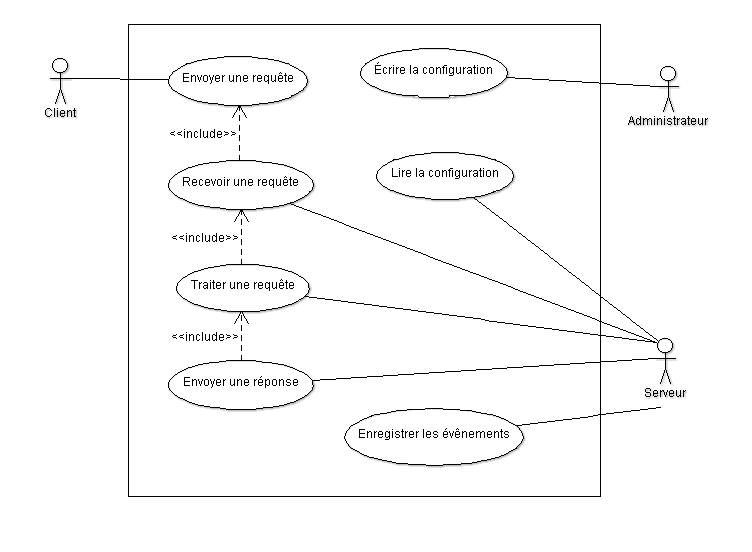
\includegraphics[width=\textwidth]{./diagram/section32.png}	
\end{figure}
\subsection{Réception d'une requête}
\subsubsection{Titre du cas d'utilisation:} Réception d'une requête
\subsubsection{Priorité:} 1
\subsubsection{Description sommaire:} Je reçois une requête et je l'envoie au module de traitement.
\subsubsection{Acteurs:}
\begin{itemize}
    \item Client
    \item Serveur
\end{itemize}
\subsubsection{Préconditions:}
\begin{itemize}
	\item Le client doit être connecté au serveur.
    \item Une requête doit avoir été envoyée par un client.
\end{itemize} 
\subsubsection{Postconditions:}
\begin{itemize}
    \item  L'information de la requête est envoyée au module de traitement.
    \item  L'événement est enregistré dans le fichier log.
\end{itemize} 
\subsubsection{Description du processus:}
Je dois pouvoir recevoir une ou plusieurs requêtes simultanément. Après l'envoie d'une requête effectuée par le client, je vais écouter un ou plusieurs port(s) à l'aide d'un socket. Ensuite, je vais identifier le type de requête qui m'a été transmis et l'assigner au module de traitement sous forme de texte.Finalement, le log enregistre l'événement.


(@TODO A Faire:DIAGRAMME
Example de requêtes;
Démontrer le traitement;
Example de retour ;
PIJI)


\subsection{Traiter une requête HTTP}
\subsubsection{Titre du cas d'utilisation:} Traiter une requête HTTP
\subsubsection{Priorité:} 2
\subsubsection{Description sommaire:} Le serveur doit traiter la requête qui lui a été assignée.
\subsubsection{Acteurs:}
\begin{itemize}
    \item Serveur
\end{itemize}
\subsubsection{Préconditions:}
\begin{itemize}
    \item On retourne une erreur si la reqûete est invalide.
    \item Doit être informé qu'une requête est prête a être traitée.  
\end{itemize} 
\subsubsection{Postconditions:}
\begin{itemize}
    \item Le traitement de la requête à été effectué.
    \item L'événement est enregistré dans le fichier log. 
    \item Retourne l'état de la requête.    
\end{itemize} 
\subsubsection{Description du processus:}En tant que Nitcorn, je dois traiter une requête HTTP qui a été reçue. Une requête HTTP doit posséder les informations suivantes :
\begin{itemize}
    \item La version du protocole HTTP
    \item Le URI
    \item Le host
\end{itemize}
Une requête doit être valide sinon on retourne une message d'erreur. Avec les informations que j'ai, je vais pouvoir lire ma configuration actuelle. Si
je trouve un virtual host correspondant au host de ma requête, je vais utiliser la configuration de ce host. Sinon je vais utiliser la configuration du host par défaut. \\
\\
Le premier élément de la configuration que je lis pour ce host est de déterminer
si, pour ce host et URI, je dois soit : lire un fichier statique, passer la requête
à une application Nit, ou passer la requête à un serveur mandataire (reverse-proxy).\\
\\
Lorsque je traite une requête pour une page statique, je dois récupérer la page par
défaut et le dossier racine pour ce host. Avec ces informations-là, je peux renvoyer
le contenu de la page statique au requérant. Si je ne suis pas en mesure de lire
la page ou le dossier demandé, je dois retourner un message d'erreur au requérant
(404-Not Found, 401-Unauthorized, etc).\\
\\
Si la requête doit être passée à un serveur mandataire, je vais créer
une requête web avec les mêmes informations que la requête, mais je vais modifier
l'argument \textit{host} pour pointer vers le host du serveur mandataire. Lorsque
la requête est envoyée, je vais attendre la réception de la réponse et transmettre
cette réponse au client.
\\
Finalement, si la requête doit être transmise à une application Nit, je vais
appeller la méthode answer de l'application en lui donnant en paramètre la requête (HttpRequest) pour communiquer avec l'application qui m'a instanciée. Par la suite, je vais attendre de recevoir la réponse de l'application
et lorsque je l'ai reçu, je vais décoder cette réponse et créer la réponse HTTP
à transmettre avec les éléments suivants :
\begin{itemize}
    \item Le code de statut HTTP
    \item La taille de la réponse
    \item D'autres \textit{headers} transmis par l'application NIT
    \item Le contenu de la réponse
\end{itemize}
Après que la réponse est transmise au client, si le protocole HTTP est 1.0, je ferme
la connexion. Si le protocole HTTP est 1.1, je dois garder la connexion
ouverte. De plus, je vais écrire un événement pour cette réponse (voir section
\textit{Enregistrer les événements}).


\subsection{Lire la configuration}
\subsubsection{Titre du cas d'utilisation:} Lire la configuration
\subsubsection{Priorité:} 4
\subsubsection{Description sommaire:}Je dois configurer le serveur à la discrétion de l'administrateur ou de l'administrateur système. 
\subsubsection{Acteurs:}
\begin{itemize}
    \item Serveur
    \item Administrateur
    \item Administrateur système
\end{itemize}
\subsubsection{Préconditions:}
\begin{itemize}
    \item On doit avoir une configuration par défaut.
\end{itemize} 
\subsubsection{Postconditions:}
\begin{itemize}
    \item On va effectuer un recherche dans la base de donnée pour récupérer la configuration la plus récente..
    \item L'événement est enregistré dans le fichier log.
    \item La configuration est changée.

\end{itemize} 
\subsubsection{Description du processus:}En tant que serveur, je vais faire une première lecture des mes configurations dans la base de données afin de connaître comment traiter les requêtes que je vais recevoir.
Pour éviter de faire une relecture dans la base de données pour chaque requête,
je vais écrire ces informations dans ma classe.
Si une application change ma configuration, je vais en tenir compte dans ma
classe pour éviter d'utiliser une configuration qui n'est plus à jour.

\subsection{Écrire la configuration}
\subsubsection{Titre du cas d'utilisation:} Écrire la configuration
\subsubsection{Priorité:} 5
\subsubsection{Description sommaire:} On cherche à changer ma configuration.
\subsubsection{Acteurs:} 
\begin{itemize}
    \item Administrateur système ou administrateur
    \item Serveur
\end{itemize}
\subsubsection{Préconditions:}
\begin{itemize}
    \item L'adminstrateur effectue un changement à la configuration.
\end{itemize} 
\subsubsection{Postconditions:}
\begin{itemize}
    \item  Le serveur est informé que la configuration à changer.
    \item  L'événement est enregistré dans le fichier log.
\end{itemize} 
\subsubsection{Description du processus:}En tant que serveur, si un administrateur change la valeur de un ou plusieurs paramètre(s)
de configuration à l'aide de l'API en fournissant des nouvelles valeurs valides,
je dois ajuster mes attributs de classe et valeurs dans la base de donnée
pour tenir compte des ajustements.

\subsection{Enregistrer les événements}
\subsubsection{Titre du cas d'utilisation:} Enregistrer les événements
\subsubsection{Priorité:} 3
\subsubsection{Description sommaire:}Je dois sauvegarder dans un fichier tous les événements.
\subsubsection{Acteurs:}
\begin{itemize}
    \item Serveur
\end{itemize}
\subsubsection{Préconditions:}
\begin{itemize}
    \item  Un fichier Log doit être créer existant sinon on le crée.
\end{itemize} 
\subsubsection{Postconditions:}
\begin{itemize}
    \item  Le fichier contient toute les informations des événements.
\end{itemize} 
\subsubsection{Description du processus:}En tant que serveur, je désire garder un historique de mes transactions. Par
défaut je respecte le \textbf{standard NCSA Common log format}\cite{NCSA}. Par contre je m'adapte
aux administrateurs, qui eux ont la possibilité de changer le format de
l'enregistrement. Mes enregistrements sont cours et concis. Ils expliquent
simplement qui a fait quoi et quand.


\section{Spécification des cas d'utilisation pour l'application Nit}


\begin{figure}[h]
\caption{Cas d'utilisation pour l'application Nit}	
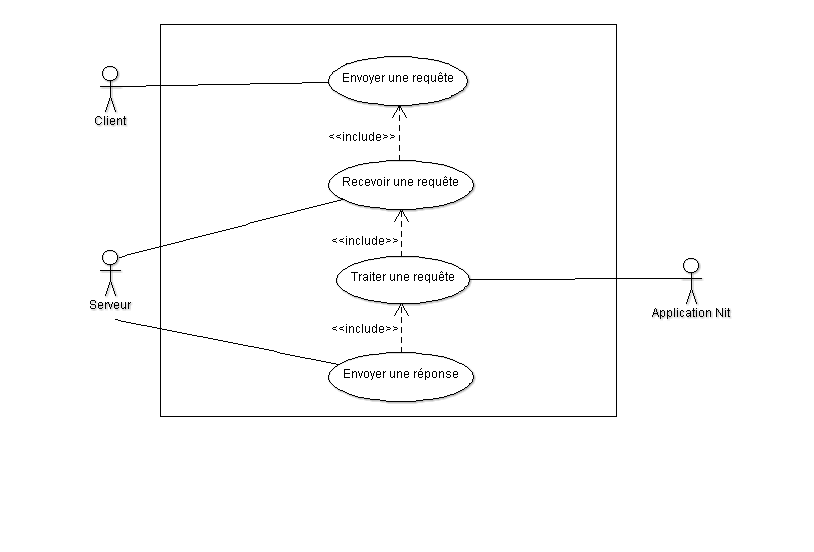
\includegraphics[width=\textwidth]{./diagram/section33.png}	
\end{figure}
\subsection{Recevoir une requête HTTP}

\subsubsection{Titre du cas d'utilisation:} Recevoir une requête HTTP
\subsubsection{Priorité:} 2

\subsubsection{Description sommaire:}
Réception d'une requête HTTP par l'application Nit via l'interface de Nitcorn.

\subsubsection{Acteurs:}
\begin{itemize}
	\item Client
    	\item Serveur
\end{itemize}

\subsubsection{Préconditions:}
\begin{itemize}
    \item Aucune.  
\end{itemize} 

\subsubsection{Postconditions:}
\begin{itemize}
    \item Le serveur doit traiter la requête reçue.
\end{itemize} 

\subsubsection{Description du processus:}
En tant qu'application Nit, je peux recevoir une requête HTTP grâce à l'interface
serveur/application me permettant de communiquer avec le serveur
Nitcorn. La réception d'une requête se fait en passant en paramètre les informations
reçu par Nitcorn (host, uri, headers).

\subsection{Traiter une requête HTTP}

\subsubsection{Titre du cas d'utilisation:} Traiter une requête HTTP
\subsubsection{Priorité:} 2
\subsubsection{Description sommaire:}
Traitement d'une requête HTTP reçue par l'application Nit.

\subsubsection{Acteurs:}
\begin{itemize}
    \item Application Nit
    \item Serveur
\end{itemize}

\subsubsection{Préconditions:}
\begin{itemize}
    \item Le serveur doit recevoir une requête HTTP. 
\end{itemize} 

\subsubsection{Postconditions:}
\begin{itemize}
    \item Le serveur doit envoyer une réponse HTTP au client. 
\end{itemize}
 
\subsubsection{Description du processus:}
Après qu'une requête HTTP a été reçue, j'achemine l'information à 
l'application destinataire qui elle fait le traitement nécessaire.

\subsection{Envoyer une réponse HTTP}

\subsubsection{Titre du cas d'utilisation:} Envoyer une réponse HTTP
\subsubsection{Priorité:} 3
\subsubsection{Description sommaire:}
Envoi d'une réponse HTTP.

\subsubsection{Acteurs:}
\begin{itemize}
	\item Client
	\item Serveur
\end{itemize}

\subsubsection{Préconditions:}
\begin{itemize}
	\item Le traitement de la requête HTTP doit être complété.
\end{itemize}

\subsubsection{Postconditions:}
\begin{itemize}
	\item Aucun.
\end{itemize}

\subsubsection{Description du processus:}
Une fois que le traitement de la requête HTTP est complété, je dois retourner une 
réponse selon de protocole de l'interface avec Nitcorn. Cette réponse doit
contenir le contenu de la réponse HTTP, mais également le code de statut HTTP
et les différents \textit{headers} HTTP.

\section{Spécification des cas d'utilisation pour API}
\subsection{Lire la configuration}
\subsubsection{Titre du cas d'utilisation:} Lire la configuration
\subsubsection{Priorité:} 6
\subsubsection{Description sommaire: A pour but d'informer l'administrateur sur les paramètres de configuration du serveur.}
\subsubsection{Acteurs:}
\begin{itemize}
	\item Administrateur système ou administrateur
    \item Serveur
\end{itemize}
\subsubsection{Préconditions:}
\begin{itemize}
    \item L'administrateur demande de l'information sur les paramètres du serveur.
\end{itemize} 
\subsubsection{Postconditions:}
\begin{itemize}
    \item  L'API retourne l'information de la configuration.    
\end{itemize} 
\subsubsection{Description du processus:}En tant qu'administrateur, si je veux savoir l'état de un ou plusieurs paramètres de
configuration sur le serveur, je vais utiliser une API pour interroger la
classe en question qui, elle, me retournera la ou les valeur(s) désirée(s).
Si j'utilise l'API pour interroger une classe à propos d'un paramètre
inexistant, je vais recevoir une erreur m'indiquant que la clé en question
n'existe pas.

\subsection{Enregistrer la configuration}
\subsubsection{Titre du cas d'utilisation:} Enregistrer la configuration
\subsubsection{Priorité:} 6
\subsubsection{Description sommaire: Va permettre au administrateur d'effectuer le changement des configurations.}
\subsubsection{Acteurs:}
\begin{itemize}
	\item Administrateur système ou administrateur
    \item Serveur
\end{itemize}
\subsubsection{Préconditions:}
\begin{itemize}
    \item On doit vérifier que la clé est valide.
    \item Vérifier que les paramètres sont valides.
\end{itemize} 
\subsubsection{Postconditions:}
\begin{itemize}
    \item On change la configuration du serveur.
    \item Si on ne peut pas changer la configuration, on affiche un message d'erreur.
\end{itemize} 
\subsubsection{Description du processus:}En tant qu'administrateur, si je désire apporter une modification à un ou plusieurs
paramètres de la configuration sur le serveur, je vais fournir la ou les nouvelle(s) valeur(s)
du ou des paramètre(s) désirée à l'API qui se chargera de relayer l'information à la classe appropriée.
Si j'essaie de faire une modification sur un paramètre qui n'existe pas sur le
serveur à l'aide de l'API, je vais recevoir une erreur m'indiquant que la clé en
question n'existe pas.
Si j'essaie de faire une modification sur un paramètre à l'aide la l'API et que
je lui fournis une valeur qui est invalide dans le contexte du paramètre, je
vais recevoir une erreur m'indiquant que le paramètre ne peut pas contenir
la valeur fournie.

\section{Exigences des interfaces externes}
\subsection{Requête HTTP}
\subsubsection{But} Le but d'une requête HTTP est de demander au serveur une ressource quelconque.
\subsubsection{Provenance} La requête HTTP est soumise par le client.
\subsubsection{Synchronisation} Le serveur Nitcorn traite les requêtes de manière asynchrone. Il n'y a donc aucune synchronisation.
\subsubsection{Rapport avec les autres intrants/extrants} Il y a une requête HTTP pour chaque réponse HTTP.
\subsection{Réponse HTTP}
\subsubsection{But} Le but d'une réponse HTTP est de fournir au client la ressource demandée.
\subsubsection{Provenance} La réponse HTTP est émise par le serveur.
\subsubsection{Synchronisation} Le serveur Nitcorn traite les réponses de manière asynchrone. Il n'y a donc aucune synchronisation.
\subsubsection{Rapport avec les autres intrants/extrants} Pour chaque réponse HTTP, il y a une requête HTTP.
\subsection{Configuration}
\subsubsection{But} Les but de la configuration est d'informer le serveur web sur la façon de traiter les requêtes HTTP.
\subsubsection{Provenance} Il y a une configuration par défaut qui sera fournie avec le serveur Nitcorn. 
\subsubsection{Synchronisation} La configuration du server ne necessite aucune synchronisation.
\subsubsection{Rapport avec les autres intrants/extrants} La configuration détermine la façon dont la requête sera traité par le serveur.
% Pour la configuration du serveur, un service web sera disponible pour configurer le serveur selon les préférences du client. (ACOMPLETE)
\section{Exigences fonctionnelles}
\begin{itemize}
    \item Lors du démarrage, le système doit lire sa configuration enregistré dans la base de données.
    \item Sur réception d'une requête, le système doit vérifier que le «Host» spécifié par le header du même nom existe dans la configuration du serveur, s'il n'existe pas
        le serveur Nitcorn utilisera un hôte par défaut.
    \item Une fois que l'hôte est trouvé, le système doit aller chercher la racine de l'hôte.
    \item Si la ressource demandée est un dossier et que le client y a accès, le système doit retourner une liste des fichiers et/ou dossiers contenus dans ce même dossier.
    \item Si la ressource demandée est un fichier et que le client y a accès, le système doit retourner le contenu du fichier dans la réponse HTTP.
    \item Si la ressource demandée est un dossier ou un fichier et que le client n'y a pas accès, le système doit retourner un code d'erreur approprié.
\end{itemize}
\section{Exigences de performance} Le serveur sera en mesure de gérer plus de 10 000 requêtes simultanées qui devront être traitée en moins de 100 millisecondes chacune. 
\section{Contraintes sur la base de données}
\subsection{Information contenue}
La base de données de Nitcorn devra contenir les informations de la configuration:
\begin{itemize}
	\item Chemins des différents fichiers de log.
	\item Les différentes données des hôtes virtuels.
\end{itemize}
\subsection{Fréquence d'utilisation}
Elle ne sera lu que lors du démarage de Nitcorn ou lors d'une modification de la configuration.
La charge qu'elle devra soutenir sera ainsi que très minime.
\subsection{Accessibilité}
Elle devra être accessible que par le serveur Nitcorn ou les administrateurs de celui-ci.
\subsection{Données}
\begin{itemize}
	\item Un chemin par fichier de log.
	\item Un nom, un port, un dossier racine et une liste d'alias par hôte virtuel.
\end{itemize}
\subsection{Rétention des données}
Le serveur Nitcorn aura besoin des données de cette base de données pour fonctionner, donc en contrepartie d'une petite charge, l'intégrité des données est primoridale. Elle ne devra donc être victime d'aucune perte de données dans la mesure du possible et devra offrir la possibilité de copier son contenu pour une sauvegarde de sûreté et d'importer une telle sauvegarde.

\section{Contraintes de conception} Le logiciel doit respecter les contraintes de conception de la norme RFC2616.
\section{Conformité avec les standards}
\subsection{Requête HTTP}
Le format et le contenu d'une requête HTTP doit être conforme avec la section 5 du RFC2616\cite{http1.0} mit en référence.
\subsection{Réponse HTTP}
Le format et le contenu d'une réponse HTTP doit être conforme avec la section 6 du RFC2616\cite{http1.0} mit en référence.
\subsection{Entrée de transaction dans le log}
Ces entrées doivent respecter le NCSA Common Log Format\cite{NCSA} tel que fournit en référence.



\section{Attributs}
\subsection{Disponibilité}
Le serveur web doit être disponible 99\% du temps entre le démarrage du serveur et jusqu'à ce que l'utilisateur le ferme.
\subsection{Sécurité}
Le serveur ne doit pas permettre d'exécution de code à distance non autorisé. Seul les usagers autorisés vont pouvoir modifier la configuration du serveur.
\subsection{Maintenabilité}
Le serveur devra pouvoir changer sa configuration sans être redémarrer.
\subsection{Transférabilité} 
Compte tenu que nitc ne supporte que les système d'exploitation de famille GNU/Linux, le serveur Nitcorn pourra seulement être déployé
sur des machines de même famille. 
Le module de persistance permettra facilement d'importer et d'exporter la configuration d'un serveur Nitcorn à un autre.

\subsection{Test}
Test de performance et de stabilité du serveur avec des utilitaires de benchmark tel que Apache Benchmark (ab) ou Siege. Puisqu'il n'existe aucune librairie de tests unitaires en Nit, chacun des modules développées auront des tests de base embarqués. ces tests ne seront aucunement aussi complet que des test unitaires.
\begin{thebibliography}{9}
\bibitem{ieefr}
  Société d'informatique IEEE,
\emph{Norme IEEE 830-1993, Pratique recommandée par IEEE pour la préparation de
spécifications d’exigences de logiciel}, 1993
\url{http://www.cours.polymtl.ca/log3410/bibliographie/IEEE/Pratique_Recommandee_Par_IEEE_pour_la\%20_Specification.pdf}.
\bibitem{c10k}
  Dan Kegel
\emph{The C10K Problem}, 1999, \url{http://www.kegel.com/c10k.html#strategies}\bibitem{http}
    The Internet Society,
\emph{Hypertext Transfer Protocol -- HTTP/1.1}, 1999,
\url{https://tools.ietf.org/html/rfc2616}
\bibitem{http1.0}
    The Internet Society,
\emph{Hypertext Transfer Protocol -- HTTP/1.0}, 1996,
\url{https://tools.ietf.org/html/rfc1945}
\bibitem{NCSA}
	NCSA,
\emph{Common Log Format},
\url{http://httpd.apache.org/docs/2.2/logs.html#common}	
\end{thebibliography}

% add other chapters and sections to suit
\end{document}
